\section{Sequences}
The next stop for us is sequences and series.  In the realm of analysis, these are very important objects.  It turns out that they are rather useful in applied sciences as well.  Specifically, power series are undeniably useful.  However, to gain understanding for those series, we need to start at the beginning with sequences.  From there, we can realize a series as a sequence.  Finally, we can turn functions into series, which, believe it or not, gives us the ability to solve problems like differential equations or to approximate harder problems in a nicer way.

\begin{df}{Sequences}{sequences}
An (infinite) \boldgreen{sequence} $\{a_n\}_{n=1}^\infty$ is an (infinite) list of numbers typically written as follows:
\[
\{a_n\}_{n=1}^\infty = a_1,~ a_2,~ a_3, \cdots.
\]
While some speak of finite sequences, we will not.  All sequences we consider are infinite, and so we drop the extra adjective.
\end{df}

Sequences can come up in all types of ways.  For example, consider these two sequences related to the number $\pi$.  We can take
\[
a_n = \textrm{the $n^\textrm{th}$ digit of the number $\pi$}
\]
and so 
\[
\{a_n\}_{n=1}^\infty = 3,~1,~4,~1,~5, \dots.
\]
We could also consider a sequence that successively approximates $\pi$ as
\[
b_n = \textrm{the $n^\textrm{th}$ decimal approximation of $\pi$}
\]
which is
\[
\{b_n\}_{n=1}^\infty = 3,~3.1, ~ 3.14, ~ 3.141, ~ 3.1415, \dots.
\]

\subsection{Convergence}
When investigating series, we often care about whether they seem to trend towards a common value or not.  This can be rather hard to deal with in some cases.  But, the intuition on when a series converges is very important and shows up in various ways one should care about.  For example, we often use computer approximations for functions (since most functions cannot be exactly calculated with a computer) and we should know when these approximations are accurate and tend towards the exact function we desire.  This motivates the following definition.

\begin{df}{Convergence of a Sequence}{convergence_of_sequence}
Consider a sequence $\{a_n\}_{n=1}^\infty$.  We say that the sequence \boldgreen{converges} to its \boldgreen{limit} $L$ if for any number $\epsilon>0$ there exists $N\in \N$ such that for any $K\geq N$ we have
\[
|a_{K}-L|<\epsilon.
\]
We then write
\[
\lim_{n\to \infty} a_n = L
\]
or
\[
a_n \to L.
\]

If a sequence does not converge to any limit, then we say the sequence \boldgreen{diverges}.
\end{df}

Admittedly, this definition is a bit obtrusive.  What is it really saying?  Let's decode this a bit. Think of $\epsilon$ as a tolerance parameter (i.e., how accurate you would like a measurement to be) telling us how far from the ideal measurement $L$ we are. Then, what this definition is saying is that if we look far enough along in our sequence we can be as close to the ideal $L$ as we wish.  

\begin{ex}{Approximations with $\pi$}{approx_pi}
Consider the two sequences $\{a_n\}_{n=1}^\infty$ and $\{b_n\}_{n=1}^\infty$ we generated for $\pi$.  Which ones converge? Let us take a look first at
\[
\{a_n\}_{n=1}^\infty = 3,~1,~4,~1,~5, \dots.
\]
Note that this sequence, if we keep looking at successive digits, does not approach any single value.  In fact, if it did approach a single value it would have to approach a decimal $0,1,\dots, 9$.  Let's say that our sequence did converge to the decimal $0$. In which case our definition of convergence would imply that if we chose a tolerance of $0.5$, then at some point in our sequence we would have 
\[
|a_K - 0|=|a_n|=a_n<\epsilon=0.5,
\]
and so all $a_n$ after some point must be equal to $0$.  But, if that was the case, then $\pi$ would not have an infinite decimal expansion! And if we had chosen another decimal, this would still mean that $\pi$ is a rational number (which we can prove it is not). Hence, $a_n$ does not converge.

Considering $\{b_n\}_{n=1}^\infty$ may be a bit easier.  We designed this sequence to continually approximate $\pi$ as we put
\[
\{b_n\}_{n=1}^\infty = 3,~3.1, ~ 3.14, ~ 3.141, ~ 3.1415, \dots.
\]
One should believe then that $b_n\to \pi$.  We can test this with our definition.  Say we let $\epsilon = 0.1$, then we want
\[
|b_K-\pi|<\epsilon = 0.1.
\]
Now, $b_n$ is defined to be the $n^\textrm{th}$ approximation of $\pi$, so if we choose $N=2$, then for $K\geq N=2$, $b_K$ has at least the first two digits of $\pi$ correctly approximated.  Then
\[
|b_K - \pi| \leq |0.0415\dots | < 0.1 = \epsilon.
\]
Similarly, we could choose $\epsilon = 0.01$ and let $N=3$.  
\end{ex}

Often we want to define sequences in a functional way.  That is, we like to specify what the $n^\textrm{th}$ term of the sequence is by a function of $n$, $f(n)$. This is typically how sequences appear and it makes working with the definition of convergence a bit more simple as we can use rules from limits that we already know.

\begin{ex}{A Sequence Given by a Function}{sequence_by_funct}
Consider the sequence $\{a_n\}_{n=1}^\infty$ where 
\[
a_n = f(n) = \frac{1}{n}.
\]
We can then write out the sequence
\[
\{a_n\}_{n=1}^\infty = 1, ~\frac{1}{2}, ~\frac{1}{3}, ~ \frac{1}{4}, \dots.
\]
It seems like numbers in this sequence get smaller and smaller in magnitude, but are never negative.  So, one may guess that $\lim_{n\to \infty} a_n = 0$.  Let us prove that this is true.  Fix some $\epsilon >0$, then we want to find an $N$ so that for all $K\geq N$ we have
\[
|a_K - 0| = |a_K|=a_K<\epsilon.
\]
Now, we have that
\[
a_K=\frac{1}{K} < \epsilon
\]
which we can rearrange 
\begin{align*}
    \frac{1}{K} & < \epsilon \\
    \iff~ \frac{1}{\epsilon} & < K.
\end{align*}
Hence, if we pick a $N\geq K>\frac{1}{\epsilon}$ we guarantee that we satisfy our tolerance condition. Thus, since we found values of $N$ that satisfy a generic tolerance condition, we know that $a_n \to 0$.

We can see a picture of what is going on here.  I'll put the $\epsilon$ as a solid red line, and graph the points $a_N$ versus $N$ as $(N, a_N)$.
        \begin{figure}[H]
    \centering
    \begin{subfigure}[h]{0.3\textwidth}
        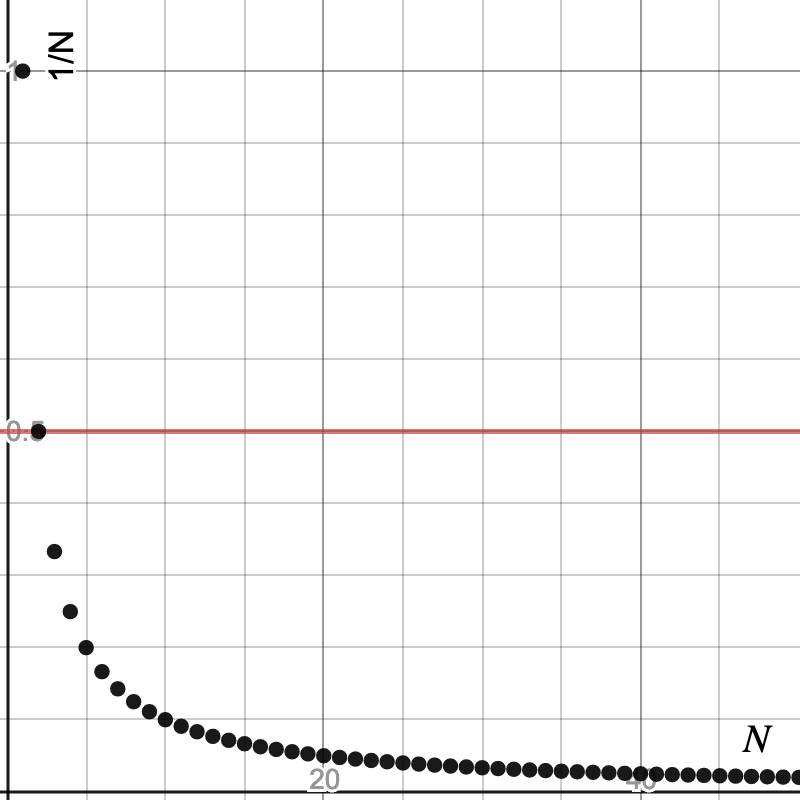
\includegraphics[width=\textwidth]{Figures_Part_3/tolerance_epsilon=05.png}
        \caption{$\epsilon=0.5$.}
    \end{subfigure}
    ~ 
    \begin{subfigure}[h]{0.3\textwidth}
        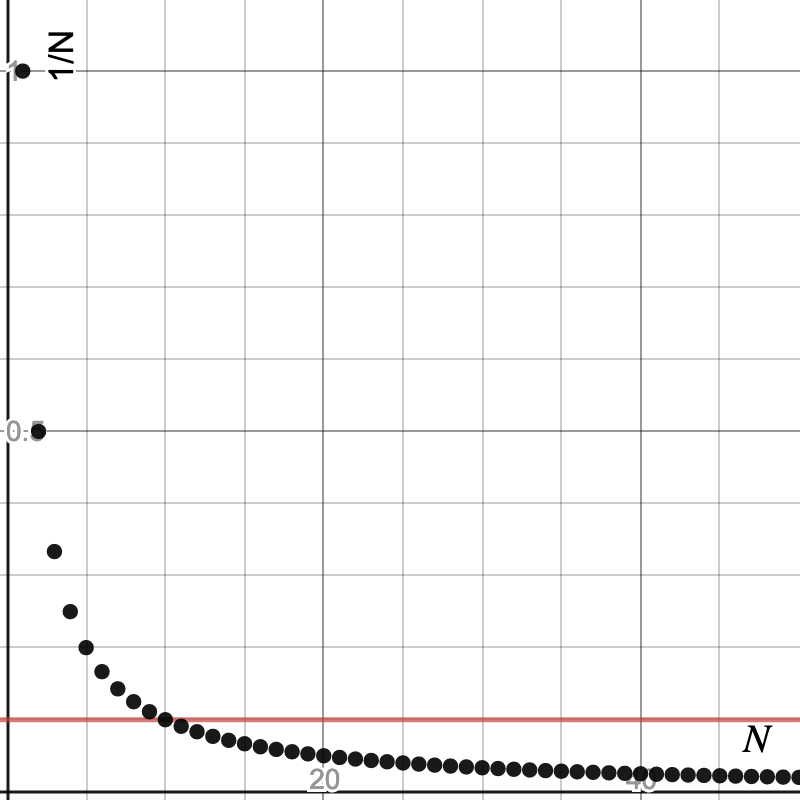
\includegraphics[width=\textwidth]{Figures_Part_3/tolerance_epsilon=01.png}
        \caption{$\epsilon=0.1$.}
    \end{subfigure}
    ~
    \begin{subfigure}[h]{0.3\textwidth}
        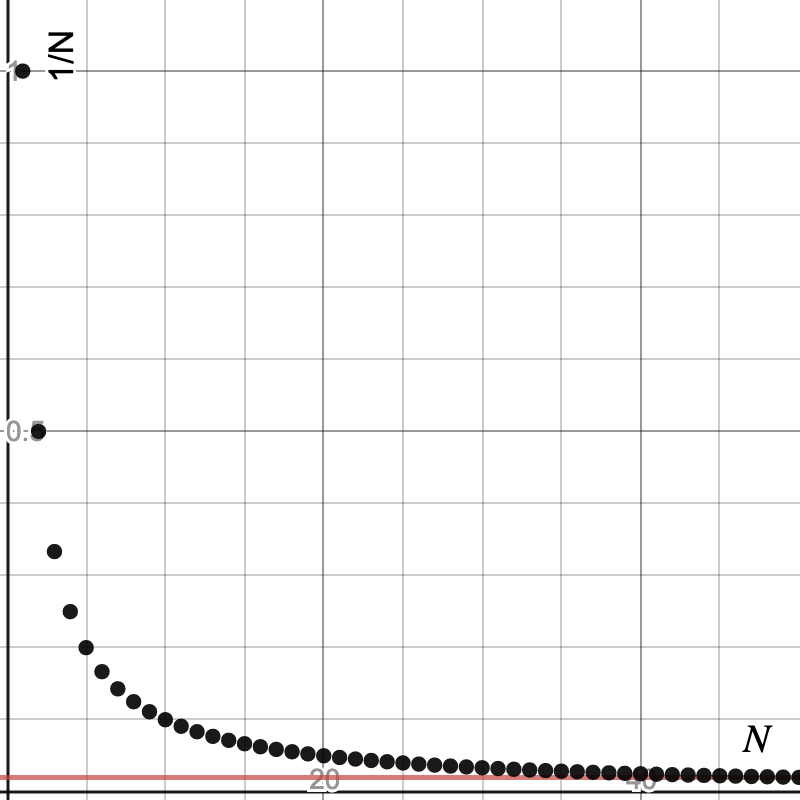
\includegraphics[width=\textwidth]{Figures_Part_3/tolerance_epsilon=002.png}
        \caption{$\epsilon=0.02$.}
    \end{subfigure}

        \end{figure}
\end{ex}

This definition of convergence is essentially the exact same definition as what we have seen for functions converging to their limit.  Hence, all the results we have on functions extends to this case.  This is why we wish to work with sequences defined by functions $f(n)$.  

\begin{prop}{Limit of Functions Gives the Limit for a Sequence}{limit_function_sequence}
Consider a sequence $\{a_n\}_{n=1}^\infty$ with $a_n = f(n)$.  Then the sequence converges to $L$ if and only if $\lim_{n\to \infty} f(n) = L$.
\end{prop}

Here's a short list of some limits you should feel free to use. 
        \begin{table}[H]
        \centering
        \renewcommand{\arraystretch}{1.75}
            \begin{tabular}{c|c}
                Function for $a_n$ &  Limit $\lim_{n\to \infty} a_n$\\
                \hline
                $a^n$ & $\begin{cases} 0 & \textrm{if $|a|<1$}\\ 1 & \textrm{if $a=1$} \\ \textrm{Diverges} &\textrm{otherwise}\end{cases}$\\
                \hline
                $n^p$ & $\begin{cases} 0 &\textrm{if $p\leq0$} \\ \textrm{Diverges} & \textrm{if $p>0$}\end{cases}$
            \end{tabular}
    \end{table}

It should be noted that not all sequences diverge in the same way.  Let us see this with an example of two different cases.

\begin{ex}{Different Ways of Diverging}{diff_diverging}
Consider the sequences $\{a_n\}_{n=1}^\infty$ and $\{b_n\}_{n=1}^\infty$ given by
\[
a_n = (-1)^n \qquad \textrm{and} \qquad b_n = n.
\]
We can write out the first few terms of each series
\begin{align*}
    \{a_n\}_{n=1}^\infty &= -1,~1,~-1,~1,~-1,~1,\dots\\
    \{b_n\}_{n=1}^\infty &= 1,2,3,4,5,6,\dots.
\end{align*}
Notice that $\{a_n\}_{n=1}^\infty$ never settles to a specific value as it just oscillates between $-1$ and $1$ indefinitely.  For $\{b_n\}_{n=1}^\infty$ we see that this sqeuence grows as $n$ grows. We sometimes add that $\{b_n\}_{n=1}^\infty$ \boldgreen{diverges to infinity}. If we took $c_n=-n$, we would have that $\{c_n\}_{n=1}^\infty$ \boldgreen{diverges to minus infinity}.
\end{ex}

Another way to describe a sequence converging is to show that the difference between successive values (i.e., differences between $a_N$ and $a_{N+1}$) get arbitrarily small.  Let us write this as a theorem. We'll define one term in this theorem as well.

\begin{thm}{Cauchy Sequences Converge}{cauchy_seq_converge}
Let $\{a_n\}_{n=1}^\infty$ be a sequence satisfying that for any $\epsilon >0$ there exists $N\in \N$ such that for $K\geq N$ we have
\[
|a_{K}-a_{K+1}|<\epsilon.
\]
We call such a sequence $\{a_n\}_{n=1}^\infty$ a \boldgreen{Cauchy sequence}.  Then if $\{a_n\}_{n=1}^\infty$ is a real (or complex) valued Cauchy sequence, then it is also convergent.
\end{thm}

\noindent This fact will become useful later on when we study series as it leads us to the comparison test.

\subsection{Recursive Sequences}

Some sequences we will see are defined in a \emph{recursive} way.  Meaning that instead of supplying a function for the terms (i.e., $a_n = f(n)$), we tend to start with an initial term $a_1$ and define future terms based on that.  For example, we could define a sequence $\{a_n\}_{n=1}^\infty$ by
\[ 
a_1 = 1 \qquad \textrm{and} \qquad a_n = \frac{1}{2} a_{n-1}.
\]
From this definition, we can find that
\[
a_2 = \frac{1}{2} a_1 = \frac{1}{2} \cdot 1 = \frac{1}{2},
\]
and
\[
a_3 = \frac{1}{2} a_2 = \frac{1}{2} \cdot \frac{1}{2} = \frac{1}{4}.
\]
If we continued on, we could write out the sequence as
\[
\{a_n\}_{n=1}^\infty = 1, \frac{1}{2},\frac{1}{4}, \frac{1}{8}, \dots.
\]
When we define a sequence in this way, we call it \boldgreen{recursive}.

\begin{ex}{Fibonacci Sequence}{fib_seq}
One very important recursive sequence is the \boldgreen{Fibonacci sequence} $\{F_n\}_{n=1}^\infty$ defined by summing up the previous two terms in the sequence to get the new one.  That is, we can define
\[
F_1 = 0, \qquad F_2=1, \qquad \textrm{and} \qquad F_n = F_{n-1} + F_{n-2}.
\]
We can write the first few terms in this sequence by following the above rule with the initial values for $F_1$ and $F_2$ to get
\[
\{F_n\}_{n=1}^\infty = 0,1,1,2,3,5,8,13,21,34,\dots.
\]
This sequence shows up in many natural systems! 
\end{ex}

\begin{exercise}
Look up where this Fibonacci sequence shows up in nature.
\end{exercise}

\section{Series}

What else can we do with sequences? Well, instead of just keeping a sequence $\seqan$ as a list of numbers, we could consider operations with these infinitely many numbers.  For example, we could add the numbers as
\[
\sum_{n=1}^\infty a_n = a_1 + a_2 + a_3 + \cdots
\]
or even multiply them
\[
\prod_{n=1}^\infty a_n = a_1\cdot a_2 \cdot a_3 \cdots.
\]
In our case, we will care about adding up terms in a sequence. 

\begin{df}{Series}{series}
Given a sequence $\seqan$ we can create an (infinite) \boldgreen{series}
\[
\sum_{n=1}^\infty a_n.
\]
\end{df}

What does it really mean to add up infinitely many numbers? Can this even be a finite result? It turns out that both of these questions can be answered at the same time.  If we rethink what we are doing a bit, it turns out that we need no other definition than convergence of a sequence.  Our goal now is to make a series into a sequence, and we will see how we can make sense of this infinite sum.

Consider a series $A=\sum_{n=1}^\infty a_n$.  We can then consider \boldgreen{partial sums} of the series by looking at finite approximations to the infinite sum.  That is, the $N^\textrm{th}$ partial sum is given by
\[
A_N = \sum_{n=1}^N a_n = a_1 + a_2 + a_3 + \cdots + a_N.
\]
Now, we can collect all of the partial sums $A_1,A_2,A_3,\dots$ and notice that this creates a sequence $\seqAn$.  

\begin{df}{Convergence of a Series}{convergence_series}
Given a series $\displaystyle{\serA}$ and the sequence of partial sums $\seqAn$. We say that the series $\serA$ \boldgreen{converges} to $A$ if the sequence of partial sums converges to $A$ and put
\[
A = \serA.
\]
If the series does not converge, we say that it \boldgreen{diverges}.
\end{df}

\begin{remark}
We should note that a series $\serA$ cannot converge if the sequence $\seqan$ does not converge to zero!
\end{remark}

\begin{ex}{Series Approximation of $\pi$}{series_approx_pi}
Previously, we had the sequences
\[
\seqan = 3,~1,~4,~1,~5, \dots
\]
and
\[
\seqbn = 3,~3.1,~3.14,~3.141,~3.1415,\dots
\]
that we used to build up the number $\pi$.  It turns out we can relate these two sequences in the following way.  Consider the series
\begin{align*}
\sum_{n=1}^\infty 10^{-n+1} a_n &= 3+0.1+0.04+0.001+0.0005+\cdots.
\end{align*}
Note, we are adding numbers of smaller and smaller magnitude. Now, notice if we take the sequence of partial sums, we find that we get back the sequence $\seqbn$
\[
b_N = \sum_{n=1}^N 10^{-n+1}a_n
\]
Since we worked with the sequence $\seqbn$ previously, we know that we have $b_n\to \pi$ and thus the series converges to $\pi$ as well
\[
\pi = \sum_{n=1}^\infty 10^{-n+1}a_n.
\]
\end{ex}

We are often provided each element of a sequence by a function. That is, $a_n=f(n)$.  If this is the case for terms in a series as well, it turns out we can use other means to show a series converges.  Let us consider the following series.

\begin{ex}{Geometric Series}{geo_series}
Consider a sequence defined by $a_n = ar^n$.  Then we call the following a \boldgreen{geometric series}
\[
\sum_{n=1}^\infty = \sum_{n=1}^\infty ar^n
\]
In order for the series to converge, we must have that the sequence $a_n \to 0$.  This means that we must have $|r|<1$ as if $|r|<1$ then $\lim_{n\to \infty} a_n =0$. If this is the case, then we can take our series
\[
\sum_{n=1}^\infty ar^n = a\sum_{n=1}^\infty r^n = a(r+r^2+r^3+\cdots).
\]
So the $N^\textrm{th}$ partial sum is
\[
A_{N} = a(r+r^2+r^3+\cdots+r^{N}).
\]
Then we can subtract $rA_N$ from both sides
\begin{align*}
A_N - rA_N &= a(r+r^2+r^3+\cdots+r^N) - a(r^2+r^3+r^4+\cdots+r^{N+1})\\
 (1-r)A_N&=a(r-r^{N+1})\\
 A_N &= a\left( \frac{r-r^{N+1}}{1-r}\right).
\end{align*}
Now consider the limit for the sequence of partial sums
\begin{align*}
\lim_{N\to \infty} A_N &= \lim_{N \to \infty} a\left(\frac{r-r^{N+1}}{1-r}\right)\\
&=\frac{ar}{1-r}.
\end{align*}
Thus, we have that the geomnetric series converges
\[
\boxed{\sum_{n=1}^\infty ar^n = \frac{ar}{1-r}.}
\]
\end{ex}

Now, not only have we shown that a whole set of series converges, but we have found what they converge to! And, as it turns out, geometric series show up quite often.  We can use our formula to find the sum of following series.

\begin{ex}{A Specific Geometric Series}{specific_geometric_series}
Consider the geometric series
\[
\sum_{n=1}^\infty \frac{1}{2^n}.
\]
Note that this is a geometric series with $a=1$ and $r=\frac{1}{2}$ as we can write the series as
\[
\sum_{n=1}^\infty a r^n = \sum_{n=1}^\infty 1\cdot \left( \frac{1}{2}\right)^n.
\]
Our formula says that
\[
\sum_{n=1}^\infty ar^n = \frac{ar}{1-r}
\]
and hence we can plug in for both $a$ and $r$ to see
\[
\boxed{\sum_{n=1}^\infty \frac{1}{2^n}=\frac{1/2}{1-1/2}=1.}
\]
\end{ex}

How about convergence for other types of series? There is a test that we can perform that will tell us more information.  We call this test the \boldgreen{ratio test}. However, the ratio test won't be a test that tells us if \emph{any} series converges or diverges.

\begin{prop}{Ratio Test}{ratio_test}
Consider the series $\serA$. If we have that 
\[
L=\lim_{n\to \infty}\left| \frac{a_{n+1}}{a_n}\right|<1,
\]
then the series converges (absolutely).  If $L>1$, then the series diverges.  If $L=1$, then we gain no information.
\begin{proof}
First, if $L>1$, then each term is growing in magnitude for this series, and thus $a_n\not\to 0$ and the series cannot converge.

If $L<1$, then at some point along our series, $N\in \N$, we have that $1>r>\left| \frac{a_{n+1}}{a_n}\right|$
\begin{align*}
\sum_{n=1}^\infty |a_n| &= \sum_{n=1}^N |a_n| + \sum_{j=N}^\infty |a_j|\\
&= A_N + \sum_{j=1}^\infty |a_{N+j}|\\
&< A_N + \sum_{j=1}^\infty r^j |a_{N+1}|\\
&= A_N +|a_{N+1}| \sum_{j=1}^\infty r^j\\
&= A_N + \frac{|a_{N+1}|r}{1-r}<\infty.
\end{align*}
Hence the series converges (absolutely).
\end{proof}
\end{prop}

\begin{remark}
A series $\serA$ \boldgreen{converges absolutely} if 
\[
\sum_{n=1}^\infty |a_n| 
\]
converges.
\end{remark}

The ratio test is a helpful tool, but it does have its shortcomings.  We can take a look at an example where the test tells us pertinent information and one where it does not.  

\begin{ex}{Series for $e$}{series_for_e}
One can actually define the number $e$ by the series
\[
e=\sum_{n=0}^\infty \frac{1}{n!}
\]
where $n!$ is the factorial function 
\[
n!=n\cdot (n-1)\cdot (n-2)\cdots 2\cdot 1
\]
and we define $0!=1$.  Now, by saying the series above equals $e$, we should think that the series converges. But we can prove this is true using the ratio test.  Consider the terms
\[
a_n = \frac{1}{n!} \qquad \textrm{and} \qquad a_{n+1}=\frac{1}{(n+1)!}=\frac{1}{(n+1)n!}.
\]
Then if we consider
\begin{align*}
    \lim_{n\to \infty} \left| \frac{a_{n+1}}{a_n}\right|&= \lim_{n\to \infty} \left| \frac{\frac{1}{(n+1)n!}}{\frac{1}{n!}}\right|\\
    &= \lim_{n\to \infty } \left| \frac{n!}{(n+1)n!}\right|\\
    &= \lim_{n \to \infty} \left| \frac{1}{n+1}\right|\\
    &= 0.
\end{align*}
Hence, by the ratio test with $L<1$, we know the series converges. And as stated above, it converges to Euler's number $e$.
\end{ex}

Below is an important class of series called \emph{$p$-series}. These and geometric series are some of the most common that we will see.  It turns out that some $p$-series converge and others diverge depending on the value for $p$. However, the ratio test gives us no information on any of them.

\begin{ex}{$p$-Series}{}
Consider a general $p$-series which has the form
\[
\sum_{n=1}^\infty \frac{1}{n^p}
\]
where $p$ can be any real number. Now, if $p\leq 0$, then we have
\[
\lim_{n \to \infty} \frac{1}{n^p}>0
\]
and the series cannot possibly converge.  However, with the ratio test for any $p$, we see that
\[
\lim_{n\to \infty} \left|\frac{a_{n+1}}{a_n}\right|=\lim_{n\to \infty} \left|\frac{\frac{1}{(n+1)^p}}{\frac{1}{n^p}}\right|  = \lim_{n\to \infty} \left| \frac{n^p}{(n+1)^p}\right| = 1.
\]
So, for any value of $p$, the ratio test tells us nothing.  However, we can show that the $p$-series does converge for certain values of $p$.
\end{ex}

\begin{exercise}
Investigate the limit in the ratio test 
\[
\lim_{n\to \infty} \left|\frac{\frac{1}{(n+1)^p}}{\frac{1}{n^p}}\right|
\]
in more detail to show that it indeed is equal to one.
\end{exercise}

There is another test we can use to determine convergence of series which will work in some cases when the ratio test does not. We call this the \boldgreen{integral test}.

\begin{prop}{Integral Test}{integral_test}
Consider the series $\sum_{n=N}^\infty$ with $a_n=f(n)$.  Then the series converges if and only if
\[
\int_{N}^\infty f(x)dx
\]
is finite. If the integral diverges, the series does as well. \emph{Note, the integral is likely not equal to the series. It only tells us whether the series converges or not!}
\end{prop}

\begin{ex}{$p$-Series Integral Test}{int_test_p_series}
Going back to the $p$-series, we need to check whether for $p>0$ the series converges as we already ruled out $p\leq 0$ cannot.  So our series in question is
\[
\sum_{n=1}^\infty \frac{1}{n^p}
\]
so our $f(n)=\frac{1}{n^p}$ and our $N=1$.  Thus we investigate the integral
\[
\int_1^\infty \frac{1}{x^p}dx.
\]
Now, if $0<p<1$, then we have
\begin{align*}
    \int_1^\infty \frac{1}{x^p}dx &= \left[\frac{1}{-p+1} x^{-p+1} \right]_1^\infty\\
    &= \infty,
\end{align*}
since $-p+1>0$ and so $x^{-p+1}$ approaches infinity as $x\to \infty$ and this integral diverges.  Hence, the $p$-series also diverges for $0<p<1$. 

For $p=1$, we find that the integral is
\[
\int_1^\infty \frac{1}{x} dx = \left[ \ln(x) \right]_1^\infty
\]
and $\ln(x)\to \infty$ as $x\to \infty$ so this integral diverges as well.  

For $p>1$, we have
\[
\int_1^\infty \frac{1}{x^p}dx = \left[ \frac{1}{-p+1}x^{-p+1}\right]_1^\infty
\]
where $-p+1<0$. Thus, in this case, $x^{-p+1}\to 0$ as $x\to \infty$ and this integral is finite!  So, we have the following result.
\[
\sum_{n=1}^\infty \frac{1}{n^p} \qquad \begin{cases} \textrm{Diverges} & \textrm{if $p\leq 1$} \\
\textrm{Converges} & \textrm{if $p>1$}\end{cases}.
\]
\end{ex}

One last useful test is to compare to series we know more about. We call this the \boldgreen{comparison test}

\begin{prop}{Comparison Test}{comparison_test}
Suppose that we have two series $\sum_{n=N_1}^\infty a_n$ and $\sum_{n=N_2}^\infty b_n$ with $a_n,b_n\geq 0$ and for some $N \in \N$ we have that for all $K\geq N$ that $a_n\leq b_n$. Then
\begin{itemize}
    \item If $\sum_{n=N_2}^\infty b_n$ is convergent, then so is $\sum_{n=N_1}^\infty a_n$.
    \item If $\sum_{n=N_1}^\infty a_n$ is divergent, then so is $\sum_{n=N_2}^\infty b_n$.
\end{itemize}
\end{prop}
